\documentclass{article}
\usepackage{amsmath}
\usepackage{amsthm}
\usepackage{pgfplots}
\usepackage[margin=1in]{geometry}
\pgfplotsset{compat=1.18}

\numberwithin{equation}{section}
\swapnumbers
\newtheorem{theorem}[equation]{Theorem}
\newtheorem{definition}[equation]{Definition}
\newtheorem{proposition}[equation]{Proposition}
\newtheorem{lemma}[equation]{Lemma}

\title{My Favorite Linear Algebra Proofs}
\author{Sean MacPherson}
\date{December 2025}

\begin{document}

\maketitle

\section{Introduction}
I recently completed my first upper-division mathematics course, a course on abstract linear algebra. I really enjoyed the course and came away with a deeper appreciation for proofs.

Looking back on the material, I find myself returning to three proofs in particular. I enjoy the first proof because it weaves together many of the course’s central abstractions—vector spaces, linear maps, isomorphisms, and quotient spaces—to prove the rank–nullity theorem, a fundamental result in linear algebra; part of the appeal is simply that I think quotient spaces are really cool. As for the second and third proofs, I was struck by how they use tools from linear algebra to answer questions that, at first glance, seem unrelated to the subject.

\section{Rank-nullity theorem}
The rank-nullity theorem is a central theorem in linear algebra. It states that the sum of the dimensions of the range and null spaces of a linear map is equal to the dimension of its domain.

\begin{figure}[h]
\centering
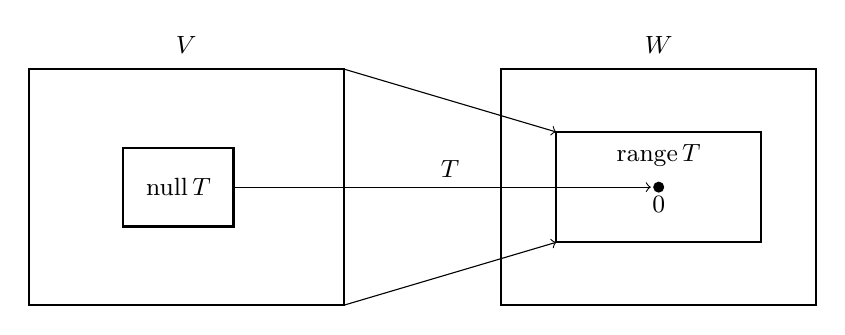
\begin{tikzpicture}[scale=1, every node/.style={font=\small}]

  % Domain V
  \draw[thick] (0,0) rectangle (4,3);
  \node at (2,3.3) {$V$};

  % Null space inside V
  \draw[thick] (1.2,1) rectangle (2.6,2);
  \node at (1.9,1.5) {$\operatorname{null} T$};

  % Codomain W
  \draw[thick] (6,0) rectangle (10,3);
  \node at (8,3.3) {$W$};

  % Range inside W
  \draw[thick] (6.7,0.8) rectangle (9.3,2.2);
  \node at (8,1.9) {$\operatorname{range} T$};

  % Zero vector centered in range
  \fill (8,1.5) circle (2pt);
  \node[below] at (8,1.5) {$0$};

  % Straight arrow: null T to 0
  \draw[->, thin] (2.6,1.5) -- (7.9,1.5);

  % Two arrows: V onto range T
  \draw[->, thin] (4,3) -- (6.7,2.2);
  \draw[->, thin] (4,0) -- (6.7,0.8);

  % Label for T
  \node[above] at (5.35,1.5) {$T$};

\end{tikzpicture}
\caption{$T: V \to W$ maps $\operatorname{null}T$ to 0 and $V$ onto $\operatorname{range} T.$}
\end{figure}

\begin{theorem}[Rank-nullity theorem]
    Let $V$ and $W$ be vector spaces with $V$ finite-dimensional, and let $T: V \to W$ be a linear map between $V$ and $W$. Then
\begin{align*}
\dim V &= \dim\mathrm{range}\ T + \dim\mathrm{null}\ T,
\end{align*}
or equivalently,
\begin{align*}
\dim V &= \mathrm{rank}\ T + \mathrm{nullity}\ T.
\end{align*}
\end{theorem}

\begin{proof}
We already have that $\text{null }T \subseteq V$, while $\mathrm{range}\ T \subseteq W$, so it is not immediately clear how to relate $\mathrm{range}\ T$ back to $V$. To address this, we will find a subspace of $V$ that is complementary to $\mathrm{null}\ T$. We will then see that T, when restricted to this complementary subspace, is an isomorphism onto $\mathrm{range}\ T$, implying that the two subspaces have the same dimension.

So how do we construct this subspace? If we work with bases and direct sums, we could extend a basis of $\mathrm{null}\ T$ to a basis of $V$, and construct this subspace as the span of the vectors that were added:
\begin{align}
\label{eq:U'}
\{\, 
\underbrace{u_1,\dots,u_k}_{\in U}
\;;\;
\underbrace{v_{k+1},\dots,v_n}_{\in U'}
\,\}
\text{ is a basis of } V,
\quad V = U \oplus U'.
\end{align}

However, there is a cleaner, basis-free way to construct this complementary subspace using the idea of a quotient space.

\begin{definition}[Quotient space]
Let $U$ be a subspace of $V$, which is finite-dimensional. The quotient space $V/U$ (``$V$ mod $U$") is given by:
\begin{align*}
V/U = \{v + U : \forall v\in V \}.
\end{align*}
Furthermore,
\begin{align}
\label{eq:quotient-dim}
\dim V = \dim V/U + \dim U.
\end{align}
\end{definition}

Each element of $V/U$ is a coset $v + U,$ which may be specified by choosing a vector $v \in V$, called a \textit{representative} of the coset.

For ease of notation, define $\pi: V \to V/U$ to be $v \mapsto v + U$, so that we may refer to elements of $V/U$ as $\pi(v)$ instead of $v + U$. Thus,
\begin{align*}
V/U = \{\pi(v): \forall v\in V \}.
\end{align*}
Note that $\pi(0)=0 + U,$ the zero element of $V/U$. One can also show that $\pi$ is a linear map whose null space is exactly $U$; that is, 
\begin{align*}
\pi(v) = 0 = \pi(0) \iff v \in U.
\end{align*}
It follows that
\begin{align}
\label{eq:pi-equality}
\pi(v)=\pi(w) \iff v-w \in U.
\end{align}

Without going into the technical details (I am now realizing how much structure goes into defining quotient spaces, much of which I either omitted or glossed over), we can think of modding out by $U$ as collapsing the directions of $V$ that lie inside $U$. In this sense, working with $V/U$ plays a role analogous to working with $U'$ from \ref{eq:U'}. Indeed, $V/U$ is isomorphic to any complementary subspace $U'$. However, $V/U$ is the more \textit{canonical} complement to $U$, since its construction does not depend on choosing a particular basis or decomposition of 
V.

Now, letting $U = \mathrm{null}\ T$ in \ref{eq:quotient-dim} gives
\begin{align*}
\dim V = \dim V/(\mathrm{null}\ T) + \dim \mathrm{null}\ T.
\end{align*}
Thus, if we can show that $\dim V/(\mathrm{null}\ T) \cong \mathrm{range}\ T$, it will follow that
\begin{align}
\label{eq:rank-nullity}
\dim V = \dim \mathrm{range}\ T + \dim \mathrm{null}\ T,
\end{align}
and the proof will be complete.

To show that $\dim V/(\mathrm{null}\ T) \cong \mathrm{range}\ T$, we must exhibit an invertible linear map between them. It turns out that $T$, acting on the quotient space $V/(\operatorname{}{null }T)$, provides exactly such an isomorphism. Accordingly, we define the map
\begin{align*}
\widetilde{T}: V/(\operatorname {null }T) \to \operatorname{range }T
\end{align*} by
\begin{align*}
\pi(v)\mapsto Tv
\end{align*}
for all $\pi(v) \in V/(\operatorname{null T}).$

To show that $\widetilde{T}$ is well-defined, suppose $\pi(v), \pi(w) \in V/(\operatorname{null}T)$ satisfy $\pi(v)=\pi(w)$. By \ref{eq:pi-equality}, this implies that $v-w\in \operatorname{null}T,$ and hence $T(v-w)=0.$ Therefore,
\begin{align*}
Tv = Tw,
\end{align*}
which shows that $\widetilde{T}(\pi(v))=\widetilde{T}(\pi(w)).$ Thus, the value of $\widetilde{T}(\pi(v))$ depends only on the coset $\pi(v),$ and not on the choice of representative $v.$ Hence, $\widetilde{T}$ is well-defined.

To show that $\widetilde{T}$ is linear, let $\pi(v),\pi(w) \in V/(\operatorname{null}T)$. $\widetilde{T}$ preserves additivity since
\begin{align*}
\widetilde{T}(\pi(v) + \pi(w)) &= \widetilde{T}(\pi(v + w)) \\
&= T(v + w) = T(v) + T(w) \\
&= \widetilde{T}(\pi(v)) + \widetilde{T}(\pi(w)),
\end{align*}
and $\widetilde{T}$ preserves homogeneity since
\begin{align*}
\widetilde{T}(\lambda\pi(v)) &= \widetilde{T}(\pi(\lambda v)) \\
&= T(\lambda v) = \lambda T(v) \\
&= \lambda \widetilde{T}(\pi(v)).
\end{align*}
Since $\widetilde{T}$ preserves additivity and homogeneity, $\widetilde{T}$ is linear.

To show $\widetilde{T}$ is an isomorphism, we must show that it is injective and surjective. To show $\widetilde{T}$ is injective, consider
\begin{align*}
0 = \widetilde{T}(\pi(v)).
\end{align*}
We must show that $\pi(v) = \pi(0).$ Expanding, we have
\begin{align*}
0 = \widetilde{T}(\pi(v)) = T(v),
\end{align*}
which implies $v \in \text{null }T = \mathrm{null}\ \pi.$ Thus, $\pi(v) = \pi(0),$ and so $\widetilde{T}$ is injective.

To show that $\widetilde{T}$ is surjective, let $w \in \mathrm{range }\ \widetilde{T}.$ We must show $\exists\pi(v) \in V/(\mathrm{null }\ T)$ such that $\widetilde{T}(\pi(v)) = w.$ Since $\mathrm{range}\ \widetilde{T} \subseteq \mathrm{range}\ T,$ $w \in \mathrm{range}\ T.$ And so $\exists v \in V$ such that $Tv = w$. This yields $$w = Tv = \widetilde{T}(\pi(v)).$$ Thus $\widetilde{T}$ is surjective.

Since $\widetilde{T}: V/(\text{null }T) \to \text{range }T$ is injective and surjective, it is an isomorphism, $\dim V/(\mathrm{null}\ T) \cong \mathrm{range}\ T$, and so the result to be shown in \ref{eq:rank-nullity} follows.

\end{proof}

\section{Existence and uniqueness of interpolating polynomial}

This next result is motivated by the following question: given a set of points with distinct x-coordinates in $\mathbf{F}^2$, does there exist a polynomial that passes through all of them?

\begin{figure}[h]
  \centering
  \begin{tikzpicture}
  \begin{axis}[
    width=8cm, height=6cm,
    axis lines=middle,
    xmin=0, xmax=10,
    ymin=0, ymax=8,
    xtick=\empty, ytick=\empty,
    xlabel={$x$}, ylabel={$y$},
    clip=false,
  ]
    % Representative points
    \addplot[
      only marks,
      mark=*,
      mark size=1.4pt
    ] coordinates {
      (1.5,2.0)
      (3.0,5.5)
      (8.5,3.5)
    };

    % Labels
    \node[anchor=north west] at (axis cs:1.5,2.0) {$\,(x_1,y_1)$};
    \node[anchor=south west] at (axis cs:3.0,5.5) {$\,(x_2,y_2)$};
    \node[anchor=north east] at (axis cs:8.5,3.5) {$(x_n,y_n)\,$};

    % Ellipsis
    \node at (axis cs:5.2,4.2) {$\cdots$};

  \end{axis}
  \end{tikzpicture}
  \caption{Is there a polynomial that passes through these points?}
\end{figure}

Regardless of the set of points, the answer is always: yes. Moreover, if we constrain the degree of polynomials we consider to one less than the number of points, there is a \textit{unique} polynomial that passes through the given points.

Using linear algebra, we can come up with a (non-constructive) proof that shows the existence and uniqueness of such a polynomial. This polynomial even has a special name: the Lagrange interpolating polynomial.

\begin{proposition}[Existence and uniqueness of interpolating polynomial]
Let $(x_1,y_1),...,(x_n,y_n) \in \mathbf{F}^2$ with $x_1,..,x_n$ distinct. Then there exists a unique polynomial $p \in \mathcal{P}_{n-1}(\mathbf{F})$ such that $p(x_1)=y_1,...,p(x_n)=y_n.$
\end{proposition}
\begin{proof}
We would like to show that there exists a polynomial $p\in\mathcal{P}_{n-1}(\mathbf{F})$ such that $p(x_1)=y_1,...,p(x_n)=y_n.$ We will construct a linear map that allows us to do this. Define $T: \mathcal{P}_{n-1}(\mathbf{F})$ by $$p \mapsto (p(x_1),...,p(x_n)).$$
From our construction of $T$, we see that $$Tp = (p(x_1),...,p(x_n)) = (y_1,...,y_n).$$

If we show that $T$ is an isomorphism, then there will be a one-to-one correspondence between polynomials in $\mathcal{P}_{n-1}(\mathbf{F})$ and vectors in $\mathbf{F}^n$ given by evaluation at $x_1,...,x_n.$ Furthermore, $T^{-1}((y_1,...,y_n))$ will be the unique polynomial, $p \in \mathcal{P}_{n-1}(\mathbf{F})$, that satisfies $p(x_1)=y_1,...,p(x_n)=y_n.$

To show that $T$ is an isomorphism, we must first show that $T$ is a linear map. Let $p,q \in \mathcal{P}_{n-1}(\mathbf{F})$ and $\lambda \in \mathbf{F}$. $T$ preserves additivity since
\begin{align*}
T(p+q) &= ((p+q)(x_1),...,(p+q)(x_n)) \\
       &= (p(x_1) + q(x_1),...,p(x_n) + q(x_n)) \\
       &= (p(x_1),...,p(x_n)) + (q(x_1),...,q(x_n)) \\
       &= Tp + Tq.
\end{align*}
Also, $T$ preserves homogeneity since
\begin{align*}
T(\lambda p) &= ((\lambda p)(x_1),...,(\lambda p)(x_n)) \\
             &= (\lambda(p(x_1)),...,\lambda (p(x_n))) \\
             &= \lambda(p(x_1),...,p(x_n)) \\
             &= \lambda Tp.
\end{align*}
Since $T$ preserves additivity and homogeneity, $T$ is linear.

Next, we must show that $T$ is injective and surjective. $T$ is a linear map between two vector spaces of the same dimension, since $$\dim \mathcal{P}_{n-1}(\mathbf{F})=\dim\mathbf{F}^n = n.$$

Thus, showing that $T$ is injective or surjective immediately implies the other. Showing that $T$ is injective is straightforward, so we will proceed with that. Consider $$Tp = ((p(x_1),...,p(x_n)) = 0 \in \mathbf{F}^n.$$ This implies that $p(x_1)=...=p(x_n)=0$, which means that $p$ has $n$ roots. By the fundamental theorem of algebra, a nonzero polynomial of degree at most $n-1$ has at most $n-1$ roots. Hence p must be the $0$ polynomial. Since $Tp=0 \implies p=0,$ $T$ is injective. It follows that $T$ is also surjective and is therefore an isomorphism.

Since $T$ is an isomorphism, $T^{-1}((y_1,...,y_n))$ is the unique polynomial of degree at most $n-1$ that satisfies $p(x_1)=y_1,...,p(x_n)=y_n.$
\end{proof}

\section{Closed-form expression for the $n$th Fibonacci number}
The $n$th Fibonacci number is usually defined using the simple recursive formula:
\begin{align}
\label{eq:fib-recurrence}
    F_n = F_{n-1}+F_{n-2}
\end{align}
where $F_0=0$ and $F_1=1.$ This yields the sequence:
\begin{align*}
    0,1,1,2,3,5,8,13,...
\end{align*}

To compute the $n$th number in the sequence, we would rather not have to compute the previous $n-1$ numbers. Fortunately, the recursion relation in \ref{eq:fib-recurrence} is linear, so we can represent it using a linear map. Furthermore, this map is diagonalizable, making it straightforward to compute a closed-form expression for the $n$th Fibonacci number. As a fun surprise, we will see that the golden ratio, $\varphi = \frac{1+\sqrt{5}}{2}$, is baked into this formula.

\begin{figure}[h]
\centering
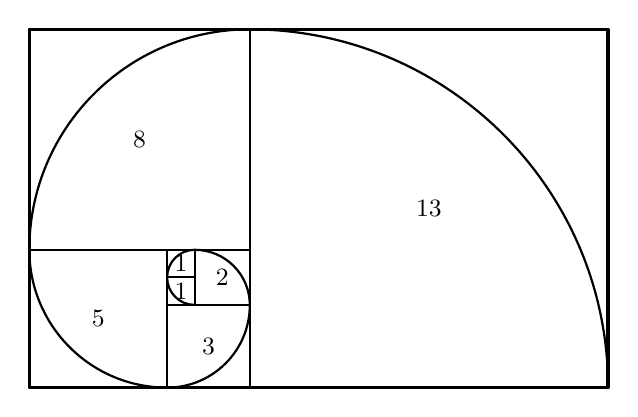
\begin{tikzpicture}[
  scale=0.35,
  line cap=round,
  line join=round,
  every node/.style={font=\small}
]

% Outer rectangle: 21 x 13
\draw[very thick] (0,0) rectangle (21,13);

% --- Fibonacci squares in the layout from your picture ---

% 13-square on the right
\draw[thick] (8,0) rectangle (21,13);
\node at (14.5,6.5) {$13$};

% 8-square top-left
\draw[thick] (0,5) rectangle (8,13);
\node at (4,9) {$8$};

% 5-square bottom-left
\draw[thick] (0,0) rectangle (5,5);
\node at (2.5,2.5) {$5$};

% 3-square (to the right of the 5-square, bottom)
\draw[thick] (5,0) rectangle (8,3);
\node at (6.5,1.5) {$3$};

% 2-square (above the 3-square, right side of the 3x2 strip)
\draw[thick] (6,3) rectangle (8,5);
\node at (7,4) {$2$};

% two 1-squares (stacked) to the left of the 2-square
\draw[thick] (5,4) rectangle (6,5);
\node at (5.5,4.5) {$1$};

\draw[thick] (5,3) rectangle (6,4);
\node at (5.5,3.5) {$1$};

% --- Golden spiral (quarter-circle arcs), clipped to outer rectangle ---
\begin{scope}
  % Outermost: in 13-square, from (21,0) to (8,13), center (21,13), radius 13
  \draw[thick] (21,0) arc[start angle=0, end angle=90, radius=13];

  % Next: in 8-square, from (8,13) to (0,5), center (0,13), radius 8
  \draw[thick] (8,13) arc[start angle=90, end angle=180, radius=8];

  % Next: in 5-square, from (0,5) to (5,0), center (0,0), radius 5
  \draw[thick] (0,5) arc[start angle=-180, end angle=-90, radius=5];

  % Next: in 3-square, from (5,0) to (8,3), center (8,0), radius 3
  \draw[thick] (5,0) arc[start angle=-90, end angle=0, radius=3];

  % Next: in 2-square, from (8,3) to (6,5), center (6,3), radius 2
  \draw[thick] (8,3) arc[start angle=0, end angle=90, radius=2];

  % Next: in top 1-square, from (6,5) to (5,4), center (5,5), radius 1
  \draw[thick] (6,5) arc[start angle=90, end angle=180, radius=1];

  % Next: in bottom 1-square, from (5,4) to (6,3), center (5,3), radius 1
  \draw[thick] (5,4) arc[start angle=-180, end angle=-90, radius=1];

\end{scope}

\end{tikzpicture}
\caption{Fibonacci tiling in a $21\times 13$ rectangle with a contained “golden spiral”.}
\end{figure}

\begin{proposition}[Formula for the $n$th Fibonacci number]
The $n$th Fibonacci number is given by
\begin{align}
\label{lem:fib-formula}
    F_n = \frac{1}{\sqrt{5}}\left[\left(\frac{1+\sqrt{5}}{2}\right)^{n} -\left(\frac{1-\sqrt{5}}{2}\right)^{n}\right].
\end{align}
\end{proposition}
\begin{proof}
Define $T: \mathbf{R}^2 \to \mathbf{R}^2$ as
\begin{align*}
    (x,y) \mapsto (y,x+y)
\end{align*}

Observe how the second component of the output vector, $x+y,$ captures the recurrence relation defined in \ref{eq:fib-recurrence}. Trivially, applying $T^0$ to $(F_0, F_1)$, which amounts to not applying $T$ at all, yields
\begin{align}
\label{eq:fib-base-case}
T^0(F_0,F_1)=I(F_0,F_1)=(F_0,F_1).
\end{align}
And as a sanity check, applying $T$ once to $(F_0,F_1)$  yields
\begin{align}
\label{eq:fib-n}
    T(F_0,F_1)=T(0,1)=(1,1)=(F_1,F_2)
\end{align}
as expected.
Thus, to compute the $n$th Fibonacci number, we should be able to repeatedly apply $T,$ then take the first component of the resultant vector:
$$T^n(F_0,F_1)=(F_n,F_{n+1}).$$
Let us prove this inductively. We have already shown that the base case, when $n=0$, holds in \ref{eq:fib-base-case}. To show the inductive case, suppose
$$T^k(F_0,F_1)=(F_k,F_{k+1}).$$
Applying $T$ to both sides gives
$$T(T^k(F_0,F_1))=T^{k+1}(F_0,F_1)=T(F_k,F_{k+1})=(F_{k+1},F_k+F_{k+1}),$$
and from \ref{eq:fib-recurrence}, we have
$$F_k+F_{k+1}=F_{k+2}.$$
Substituting, we have
$$T^{k+1}(F_0,F_1)=(F_{k+1},F_{k+2}), $$ and so the inductive case also holds. Thus
$$T^n(F_0,F_1)=(F_n,F_{n+1})$$
for all $n \in \mathbf{N}.$

Next, we will diagonalize $T$ to reduce the computation needed to take powers of $T$ to taking powers of its eigenvalues. To find $T$'s eigenvalues, we must find $\lambda\in\mathbf{R}$ satisfying
$$T(x,y)=\lambda (x,y)=(\lambda x,\lambda y)=(y,x+y)$$
Substituting $y=\lambda x$ into $x + y = 
\lambda y$ gives
\begin{align*}
    0 = \lambda^2x - \lambda x - x &= x(\lambda^2-\lambda - 1),
\end{align*}
and completing the square gives
\begin{align*}
    (\lambda^2-\lambda - 1) &= (\lambda - \frac{1}{2})^2 -\frac{5}{4} \\
    &= (\lambda - \frac{1}{2})^2 -(\frac{\sqrt{5}}{2})^2 \\
    &= (\lambda - \frac{1-\sqrt{5}}{2})(\lambda - \frac{1+\sqrt{5}}{2}).
\end{align*}
Thus, $\lambda_1=\frac{1+\sqrt{5}}{2}$ and $\lambda_2=\frac{1-\sqrt{5}}{2}.$

To find $T$'s eigenvectors, we must solve
\begin{align}
\label{eq:fib-eigenvectors}
T(x,y) = \frac{1\pm\sqrt{5}}{2}(x,y) = (y,x+y).
\end{align}
This yields the system
\[
\begin{cases}
\displaystyle \frac{1\pm\sqrt{5}}{2}\,x = y, \\[6pt]
\displaystyle \frac{1\pm\sqrt{5}}{2}\,y = x + y.
\end{cases}
\]
Since the two equations end up describing the same relationship, the first equation implies that, for any $x\in \mathbf{R},$
$$(x,\frac{1\pm\sqrt{5}}{2}\,x)$$ satisfies \ref{eq:fib-eigenvectors}. Thus, using $x=1$, we have two eigenvectors,
$b_1 =(1,\frac{1+\sqrt{5}}{2})$, corresponding to $\lambda_1$, and
$b_2 = (1,\frac{1-\sqrt{5}}{2})$, corresponding to $\lambda_2.$

Since these eigenvectors correspond to two distinct eigenvalues, they are linearly independent, and therefore form a basis of $\mathbf{R}^2,$ which we define as $\beta = \{b_1,b_2\}.$ Now letting $(x_{\beta},y_{\beta})$ be the $\beta$-coordinates of $(x,y)$, we have
\begin{align}
\label{eq:fib-map-diag}
T^n((x_{\beta},y_{\beta})) &= T^n(x_{\beta}b_1 + y_{\beta}b_2) \\
                 &= x_{\beta}T^nb_1 + y_{\beta}T^nb_2 \\
                 &= x_{\beta}\lambda_1^nb_1 + y_{\beta}\lambda_2^nb_2.
\end{align}
Now, observe that $(F_0,F_1)=(0,1)$ written in terms of $\beta$ is given by
$$
    (F_0,F_1)=(0,1) = \frac{1}{\sqrt{5}}b_1 - \frac{1}{\sqrt{5}}b_2,
$$
and so $(x_{\beta},y_{\beta})=(\frac{1}{\sqrt{5}},-\frac{1}{\sqrt{5}}).$
Substituting the values for $(x_{\beta},y_{\beta})$, $\lambda_1,\lambda_2$, and $b_1,b_2$ into \ref{eq:fib-map-diag} gives
\begin{align*}
T^n(x_{\beta},y_{\beta}) &= T^n(\frac{1}{\sqrt{5}},-\frac{1}{\sqrt{5}}) \\
    &= T^n\left( \frac{1}{\sqrt{5}}(1,\frac{1+\sqrt{5}}{2}) - \frac{1}{\sqrt{5}}(1,\frac{1-\sqrt{5}}{2})\right) \\
    &= \frac{1}{\sqrt{5}}\left(\frac{1+\sqrt{5}}{2}\right)^n(1,\frac{1+\sqrt{5}}{2}) - \frac{1}{\sqrt{5}}\left(\frac{1-\sqrt{5}}{2}\right)^n(1,\frac{1-\sqrt{5}}{2}) \\
    &= (F_n, F_{n+1})
\end{align*}
And at last, when we compute the first component, we see that
\begin{align*}
F_n = \frac{1}{\sqrt{5}}\left[\left(\frac{1+\sqrt{5}}{2}\right)^n - \left(\frac{1-\sqrt{5}}{2}\right)^n\right].
\end{align*}
\end{proof}

\end{document}
